\documentclass[oneside,14pt]{book}

\usepackage[T1,T2A]{fontenc}
\usepackage[utf8]{inputenc}
\usepackage[english,russian]{babel}
\usepackage{indentfirst}

%\usepackage[paperwidth=15cm,paperheight=7.5cm]{geometry} % планшет
%\usepackage[paperwidth=297mm,paperheight=210mm]{geometry} % A4
%\usepackage[paperwidth=148mm,paperheight=105mm]{geometry} % A5
\usepackage[paperwidth=18cm,paperheight=13cm,margin=5mm]{geometry} % экран*2

%\usepackage[colorlinks=true,
%]{hyperref}
%\newcommand{\email}[2]{#1\ \href{mailto:#2}{<\nolinkurl{#2}>}}
% %\newcommand{\email}[2]{\emph{#1\ <#2>}}
\usepackage[unicode,colorlinks,
pdftitle={Azbuka ARMaturschika (ru)},
pdfauthor={(c) Dmitry Ponyatov <dponyatov@gmail.com>, SSAU ASCL},
pdfsubject={ru manual on writing programs for Cortex-M MCUs},
pdfkeywords={ARM} {Cortex} {MCU} {ARMatura} {Arduino} {SSAU}
]{hyperref}

\usepackage{wrapfig}
\usepackage{graphicx}
\usepackage{epstopdf}
\DeclareGraphicsExtensions{.eps}

\usepackage{listings}
\usepackage{dirtree}
\usepackage[usenames,dvipsnames,svgnames]{xcolor}
\newcommand{\cppcolor}{\color[rgb]{0.94, 0.97, 1.0}} % Alice blue
\newcommand{\asmcolor}{\color[rgb]{0.98, 0.92, 0.84}} % Antique white
\newcommand{\ldcolor}{\color[rgb]{0.67, 0.9, 0.93}} % Blizzard Blue
\newcommand{\concolor}{\color[rgb]{0.88, 1.0, 1.0}} % Light cyan
\newcommand{\makecolor}{\color[rgb]{0.9, 0.9, 0.98}} % Lavender mist

%\definecolor{cppcolor}{rgb}{0.94, 0.97, 1.0}
\lstset{frame=single,
numbers=left, numberstyle=\small, numbersep=1mm,
tabsize=4,
keywordstyle=\color{blue}\texttt,
commentstyle=\color{cyan}\texttt,
inputencoding=utf8, extendedchars=true, showspaces=false,  
inputencoding=cp1251
}
\usepackage{lstlangarm}
\usepackage{lstlanggnumake}
\usepackage{lstlanggnuld}
\usepackage{lstlanggnudump}

\lstdefinestyle{cpp}{language=C++,backgroundcolor=\cppcolor}
\lstdefinestyle{asm}{language={[ARM]Assembler},backgroundcolor=\asmcolor}
\lstdefinestyle{gnuld}{language={[GNU]Link},backgroundcolor=\ldcolor}
\lstdefinestyle{con}{backgroundcolor=\concolor}
\lstdefinestyle{mk}{language=[GNU]Make,backgroundcolor=\makecolor}
\lstdefinestyle{objdump}{language=[GNU]Dump}

\newcommand{\cm}[1]{Cortex-M#1}
\newcommand{\cx}{\cm{x}}

\newcommand{\vld}{STM32VLDISCOVERY}

%\renewcommand{\url}[1]{\textbf{#1}}
\newcommand{\email}[1]{$<$\href{mailto:#1}{\textbf{#1}}$>$}

\newcommand{\cpp}{$C^{+^{+}}$}

\newcommand{\cp}[1]{\footnote{копипаста: #1}}

\newcommand{\thmod}{Thumb}
\newcommand{\armod}{ARM}
\newcommand{\arm}{ARM}

\newcommand{\Reg}[1]{\textbf{#1}}
\newcommand{\R}[1]{\Reg{R#1}}

\newcommand{\periph}[1]{\texttt{#1}}
\newcommand{\jtag}{\periph{JTAG}}

\usepackage{wasysym} % smileys
\usepackage{gensymb} % celsius
\usepackage{amssymb} % windows key
\usepackage{textcomp} % bigcircle

\usepackage[os=win]{menukeys}
\newcommand{\winstart}{$\boxplus$}
\newcommand{\file}[1]{\textbf{\textsf{#1}}}
\newcommand{\window}[1]{\textbf{\textit{#1}}}
\newcommand{\alarm}[1]{{\color{DarkRed}#1}}
\newcommand{\wcmd}[1]{\keys{\winstart+R}\ \directory{#1}}
\newcommand{\checkbox}{$\boxtimes$}
\newcommand{\uncheckbox}{$\square$}
\newcommand{\lms}{\keys{$\lhd$}}
\newcommand{\rms}{\keys{$\rhd$}}
\newcommand{\eclpx}{\window{Project Explorer}}

\newcommand{\win}[1]{
\includegraphics[height=10ex]{fig/winlogo.jpg} #1}
\newcommand{\lin}[1]{
\includegraphics[height=10ex]{fig/linuxcolor.png} #1}
\newcommand{\bug}{
\includegraphics[height=10ex]{fig/iconbug.png}}

\newcommand{\linux}{Linux}
\newcommand{\git}{Git}
\newcommand{\eclipse}{\textcircled{$\equiv$}\textsc{eclipse}}
%\newcommand{\term}[1]{\underline{#1}}
\newcommand{\term}[1]{\underline{\color{DarkBlue} #1}}
\newcommand{\miktex}{MiK\TeX}
\newcommand{\internet}{Internet}
\newcommand{\ql}{Quantum$^{\circledR}L^{e}aPs$}
\newcommand{\gdb}{GDB}

\newcommand{\make}{\file{make}}
\newcommand{\makefile}{\file{Makefile}}

\usepackage{tocloft}
\newcommand{\listlabname}{Лабораторные работы}
\newlistof{lab}{ex}{\listlabname}
\newcommand{\labpart}[1]{\addcontentsline{ex}{part}{#1}}
\newcounter{labworkcounter}
\newcommand{\labwork}[1]{
\refstepcounter{labworkcounter}
\section*{ЛР\thelabworkcounter: #1}
\addcontentsline{toc}{subsection}{ЛР\thelabworkcounter: #1}
\addcontentsline{ex}{section}{ЛР\thelabworkcounter: #1}
}
\newcommand{\labref}[1]{ЛР\ref{#1}}

\newcommand{\thetitle}{Азбука халтурщика-ARMатурщика}

\newcommand{\mytitle}[1]{
\title{\Huge{\thetitle}\\
#1\\
\normalsize{учебный курс по микроконтроллерам \cx:\\
Миландр 1986ВЕ, STM32F, LPC21xx}}
}

\author{(copypasta) Понятов Д.А. \email{dponyatov@gmail.com}, ИКП СГАУ}


\begin{document}

\section{Общая структура рабочей среды разработчика встроенных систем}

\begin{itemize}
  \item Операционная система с набором типовых утилит
  
  Для Windows требуется дополнительно установить несколько модулей из пакета
  \file{GnuWin32}, чтобы обеспечить минимальную совместимость с UNIX-средой.
  
  \item Текстовый редактор или интегрированная среда разработки (IDE)
  
  Редактирование текстов программ и скриптов сборки (компиляции) с
  цветовой подсветкой синтаксиса (в зависимости от языка файла),
  \term{автодополнением}\ и вызовом программ-утилит нажатием сочетаний 
  клавиш. Например нажатием \keys{F3}\ в \eclipse\ можно переместится на
  определение функции, на имени которой находится текствый курсор.
  
  Автодополнение\ --- редактор предлагает варианты полного написания
  идентификаторов и ключевых слов по первым буквам и нажатию обычно
  \keys{Ctrl+Tab} или \keys{Ctrl+N}. Также автоматически расставляются
  закрывающие скобки, закрывающие операторы управляющих структур типа begin/end,
  и генерируются синтаксические элементы циклов при вводе ключевых слов
  if/for/while. Особенно удобно автодополнение при написании кода на ООП 
  языках\  --- при вводе имени класса или объекта и точки предлагается меню с
  именами данных и методов класса. 
  
  При вводе имени функции и скобки выводится всплывающее окно с подсказкой\ ---
  определение функции с типом возвращаемого значения, типом и именами
  параметров.
  
  Интерфейс IDE часто предусматривает различные вспомогательные окна,
  показывающие имена и свойства объектов, описанных в программе (переменные,
  функции, структуры,..), структуру проекта с зависимостями между файлами, блоки
  справки в зависимости от текущего выделенного элемента и т.п.
  
  Часто IDE имеет встроенный графический интерфейс для отладки программ,
  используя для этого интерфейсные библиотеки для программатора и
  специальный отладочный код, добавляемый к вашей программе при
  компиляции. Используя аппаратный модуль отладки на целевом процессоре и
  отладочный код, IDE обеспечивает отображение значений и изменений регистров
  процессора, состояние переферии, позволяет задать точки останова в программном
  коде, в т.ч. условные по значению или измениею переменных или регистров
  железа.
  При использовании ОС реального времени и системы аппаратной многозадачности
  отображается загрузка ядер, загрузка процессора и используемые ресурсы для
  каждой задачи, работа планировщика, и т.п.
  
  \item Пакет кросс-компилятора и утилит типа make, objdump,..
  
  Компилятор преобразует программы на языке программирования в \term{объектный
  код} (смесь кусочков машинного кода со служебной информацией) или в
  текст на языке ассемблера.
  
  \term{Кросс-компилятор}\ (arm-none-eabi-gcc) отличается от обычного
  компилятора тем, что генерирует код не для компьютера на котором он выполняется
  (\term{хост-система}, \verb|$HOST|), а для компьютера другой
  архитектуры\ --- \term{целевой} системы, \verb|$TARGET|.
  
  \term{Ассемблер}\ (as) преобразует человекочитаемый код программы в объектный
  код.
  
  \term{Линкер}\ (ld) объединяет несколько файлов объектного кода в один,
  и корректирует машинный код с учетом его конечного размещения в памяти
  целевой системы (адреса переменных, адреса переходов, размещение сегментов
  кода и данных в физической памяти целевой системы).
  
  \term{Дампер}\ (objdump) преобразует сегменты кода/данных из файла,
  полученного линкером, в формат, необходимый для ПО программатора: бинарные файлы, Intel
  HEX, ELF,.. загружаемые в масочное ПЗУ, FlashPROM (и EEPROM данных на МК
  ATmega).
  
  \item ПО для программатора, JTAG-адаптера
  
  Загрузка полученной прошивки в целевое устройство, редактирование памяти, 
  внутрисхемная отладка в процессе работы устройства, прямое измение сигналов на
  выводах процессора (граничное сканирование и тестирование железа).
  
\end{itemize}

\win{\labwork{Установка IDE}\label{winide}}

Для удобной работы доступно несколько бесплатных вариантов IDE (интегрированных сред разработки),
рассмотрим два варианта: тяжелая суперуниверсальная среда Eclipse, и легкая в отношении требуемых
ресурсов системы CodeLite.

\bigskip Для работы Eclipse требуется установленная Java:

\bigskip\wcmd{\url{http://www.oracle.com/technetwork/java/javase/downloads/}}

\bigskip\begin{itemize}
  \item 
Минимальный вариант\ ---  ставим только Java Runtime:

\menu{Java Platform, Standard Edition>JRE>Download>Accept
License>\file{jre-8u5-windows-i586.exe}}

\menu{\file{jre-8u5-windows-i586.exe}>Welcome>\checkbox\ Change destination
folder>Install}

\menu{Destination folder>\file{D:/Java/jre8}>Next>Installing>Close}

  \item
Если вы планируете параллельно еще и осваивать язык Java\ --- ставим
Java SE JDK: 

\menu{Java Platform, Standard Edition>JDK>Download>Accept
License>\file{jdk-8u5-windows-i586.exe}}

\menu{\file{jdk-8u5-windows-i586.exe}>Welcome>Next}

\menu{Install to: \file{D:/Java/jdk8}>Next}

\menu{JRE Distination folder>Install to: \file{D:/Java/jre8}>Next}

\menu{Java SE Development Kit 8 Update 5 Successfully Installed>Close}

\end{itemize}

Для установки доступны два варианта:
\begin{enumerate}
\item \textbf{Eclipse Standard} базовый вариант среды, в ЛР рассмотрен именно он для иллюстрации 
ручной установки расширений
\item \textbf{Eclipse IDE for C/C++ Developers} вариант сборки 
уже включает расширение CDT, поэтому в следующий раз рекомендуем сразу качать его,
это упростит и съэкономит немного времени на установку рабочей среды
\end{enumerate}

\bigskip\wcmd{\url{http://www.eclipse.org/downloads/}}

\bigskip\menu{Eclipse Standard>Windows 32
Bit>Download>\file{eclipse-standard-luna-R-win32.zip}}

\bigskip Перетащите каталог \file{eclipse} из архива в \file{D:/ARM} и
создайте удобным для вас способом ссылку на \file{D:/ARM/eclipse/eclipse.exe}.

\bigskip
\includegraphics[height=0.3\textheight]{fig/EclipseSplash.png}

\bigskip Workspace\ --- рабочий каталог, в котором создаются каталоги отдельных
проектов, типа \file{D:/WORK}. Eclipse создаст в нем служебный каталог
\file{.metadata}, и поместит в него служебную информацию, относящуюся сразу ко
всем проектам. Как побочный эффект, если в workspace уже есть какой-то каталог,
можно создать новый проект (например \file{book}), и в левой части рабочей
области \eclipse\ в окне \window{Project Explorer}\ появится дерево файлов
\file{book/*}.

\bigskip\menu{\file{D:/ARM/eclipse/eclipse.exe}>Workspace>\file{D:/ARM}>Use as
default>OK}

\bigskip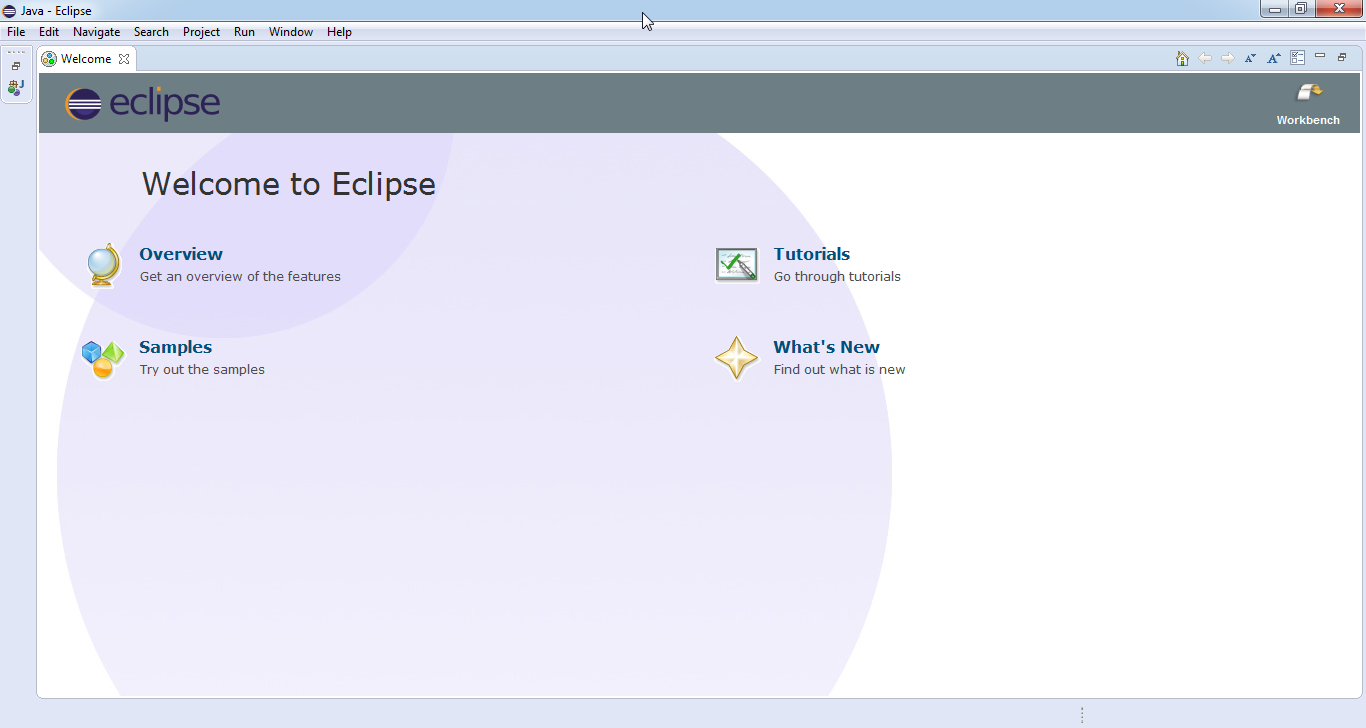
\includegraphics[width=0.9\textwidth]{fig/EclipseMain.png}

\bigskip Проверяем наличие обновлений

\bigskip\menu{Help>Check for Updates>Details>No updates found>OK}

\bigskip В базовом варианте Eclipse поддерживает только Java, поэтому нужно
установить расширение для работы с С/C++: \file{CDT}.

\bigskip
Проект \file{CDT}\ предоставляет полнофункциональную интегрированную среду
для разработки на Си и \cpp. Поддерживаются: управление проектами и
компиляцией для различных тулчейнов, стандартная сборка через
\file{make}, навигация по исходным текстам, различные инструменты для
работы с иходным текстом, такие как иерархия типов, граф вызовов, браузер
подключаемых файлов, браузер макроопределений, редактор кода с подсветкой
синтаксиса, сворачивание синтаксических структур (фолдинг) и гипертекстовая
навигация, рефакторинг и генерация кода, средства визуальной отладки,
включающие просмотр памяти, регистров и дизассемблер.

\bigskip\wcmd{\url{http://www.eclipse.org/cdt/downloads.php}}

\bigskip Выделить и скопировать в буфер обмена ссылку

\file{p2 software repository}:
\url{http://download.eclipse.org/tools/cdt/releases/8.4}.

\bigskip Добавляем сетевое хранилище пакетов для \eclipse:

\bigskip\menu{\eclipse>Help>Install New Software>Work with>Add}

\bigskip\menu{Name>CDT}

\menu{Location>http://download.eclipse.org/tools/cdt/releases/8.4}

\menu{OK}

\bigskip
Выбрать (если оно не выбралось само) хранилище \menu{Work with:>CDT},
и в дереве выбора пакетов выбрать:

\bigskip
\dirtree{%
.1 CDT.
.2 CDT Main Features.
.3 \checkbox\ C/C++ Development Tools.
.2 CDT Optional Features.
.3 \checkbox\ C/C++ C99 LR Parser.
.3 \checkbox\ C/C++ GCC Cross Compiler Support.
.3 \checkbox\ C/C++ GDB Hardware Debugging.
}

\bigskip
\menu{Next>Next>Licenses>Accept>Finish}

\bigskip После установки пакетов появится окно с запросом перезапуска \eclipse.

\bigskip Аналогично ставим плагин GNU ARM Eclipse:

\bigskip
\menu{Help>Install>Work with>Add}

\menu{Name>GNU ARM plugin}

\menu{Location>\url{http://sourceforge.net/projects/gnuarmeclipse/files/Eclipse/updates/}}

\dirtree{%}
.1 GNU ARM C/C++ Cross Development Tools.
.2 \checkbox\ Cross Compiler Support.
.2 \checkbox\ Generic Cortex-M Project Template.
.2 \checkbox\ STM32Fx Project Templates.
.2 \checkbox\ OpenOCD Debugging Support.
}

\menu{Warning: You install unsigned content>Ok}

\bigskip
В \eclipse\ есть так называемые \term{перспективы} (perspective)\ --- это
переключаемые режимы отображения рабочего набора окон, настроенные под тип
работы. По умолчанию запускается перспектива \window{Java}. Нас
интересует перспектива \window{C/C++}:

\bigskip\menu{Window>Open Perspective>Other>C/C++>Ok}

\bigskip Также перспективу можно переключить кнопкой на панели в правом верхнем
углу:

\bigskip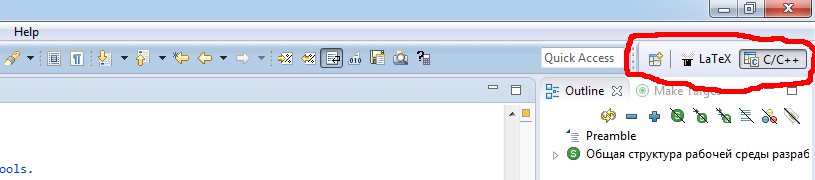
\includegraphics[width=0.9\textwidth]{fig/eclperpective.png}

\addcontentsline{toc}{part}{Литература}
\begin{thebibliography}{9}

\bibitem{leaps}{\copyright\ Quantum Leaps}

\bibitem{milandr}{\url{http://milandr.ru/} ЗАО <<ПКК Миландр>>}

\bibitem{progit}{\url{http://git-scm.com/book/ru} перевод:
Scott Chacon
\textbf{Pro Git}
}

\bibitem{habraQP}{\url{http://habrahabr.ru/post/114239/} хабра: Quantum Leaps QP
и диаграммы состояний в UML}

\bibitem{quantumleaps}{\url{http://www.state-machine.com/}
Quantum$^{\circledR}L^{e}aPs$ State Machines \& Tools}

\end{thebibliography}


\end{document}
